\documentclass[twocolumn, 10pt, conference]{IEEEtran}

% packages start
\usepackage{graphicx}
\usepackage[caption=false,font=footnotesize]{subfig}
\usepackage{algorithm}
\usepackage{algorithmic}
\usepackage{listings}
\lstset{language=Python}
\usepackage{amsmath}
\usepackage{fixltx2e} % ensures float ordering is preserved
\usepackage{url}
\usepackage{breqn}
\usepackage{cite} % orders multiple citations
\usepackage{booktabs}

\usepackage{balance}
\usepackage{lipsum}

%\usepackage{hyperref} % citations and references are hyperlinks

%\usepackage[table,xcdraw]{xcolor} % colors on tables

\usepackage{siunitx}

% the following lines cause
%\usepackage{enumitem}
%\setlist{noitemsep,topsep=2pt,parsep=2pt,partopsep=0pt}


\IEEEoverridecommandlockouts

\begin{document}

\hyphenation{VA-NET}
\hyphenation{VA-NETs}
\hyphenation{pa-th--fin-ding}
\hyphenation{heu-ris-tic--dri-ven}
\hyphenation{match-es}
\hyphenation{rang-es}
\hyphenation{mea-sure-ments}
\hyphenation{ge-o-graph-ic}
\hyphenation{to-pol-o-gy-based}



%
% --- Author Metadata here ---
%\conferenceinfo{SIGMETRICS2016}{2016 Juan-les-Pins, France}
%\CopyrightYear{2016} % Allows default copyright year (20XX) to be over-ridden - IF NEED BE.
%\crdata{0-12345-67-8/90/01}  % Allows default copyright data (0-89791-88-6/97/05) to be over-ridden - IF NEED BE.
% --- End of Author Metadata ---

\title{Experimental study on round trip times of web applications}

%
% You need the command \numberofauthors to handle the 'placement
% and alignment' of the authors beneath the title.
%
% For aesthetic reasons, we recommend 'three authors at a time'
% i.e. three 'name/affiliation blocks' be placed beneath the title.
%
% NOTE: You are NOT restricted in how many 'rows' of
% "name/affiliations" may appear. We just ask that you restrict
% the number of 'columns' to three.
%
% Because of the available 'opening page real-estate'
% we ask you to refrain from putting more than six authors
% (two rows with three columns) beneath the article title.
% More than six makes the first-page appear very cluttered indeed.
%
% Use the \alignauthor commands to handle the names
% and affiliations for an 'aesthetic maximum' of six authors.
% Add names, affiliations, addresses for
% the seventh etc. author(s) as the argument for the
% \additionalauthors command.
% These 'additional authors' will be output/set for you
% without further effort on your part as the last section in
% the body of your article BEFORE References or any Appendices.

% double-blind submission

\author{
Rafi Khaled, Rui Meireles
\\ 
\small{\texttt{\{rkhaled, rui.meireles\}@vassar.edu}}
\\ \\
\small \IEEEauthorblockA{Department of Computer Science, Vassar College, USA}
}

\maketitle
%\thispagestyle{plain} % enables page numbers
%\pagestyle{plain} % enables page numbers

%\category{C.2.2}{Computer-Communication Networks}{Network Protocols}[Routing protocols]
%\keywords{Vehicular networks, Multi-hop, Routing, Forwarding}

\setlength{\belowdisplayskip}{10pt} \setlength{\belowdisplayshortskip}{10pt}
\setlength{\abovedisplayskip}{10pt} \setlength{\abovedisplayshortskip}{10pt}
\setlength{\textfloatsep}{10pt plus 1.0pt minus 2.0pt}
\setlength{\floatsep}{10pt plus 1.0pt minus 2.0pt}
\setlength{\intextsep}{10pt plus 1.0pt minus 2.0pt}

\begin{abstract}
% motivation, problem statement, approach, results
Replace by concrete abstract.
\end{abstract}


\section{Introduction}
\label{sec:introduction}

% The introduction is very important. By the time the reviewer finishes the 
% introduction, he probably has his mind made up already: he'll read the rest 
% of the paper looking for evidence to support his decision.

% what is the problem and why is it importantly
% why is the problem hard?
% what is wrong with existing solutions?
% what do we propose to do and why is it better (i.e. what are our contributions)?

Introduction.

Figure~\ref{fig:example} is an example figure.

\begin{figure}[t]
\centering
    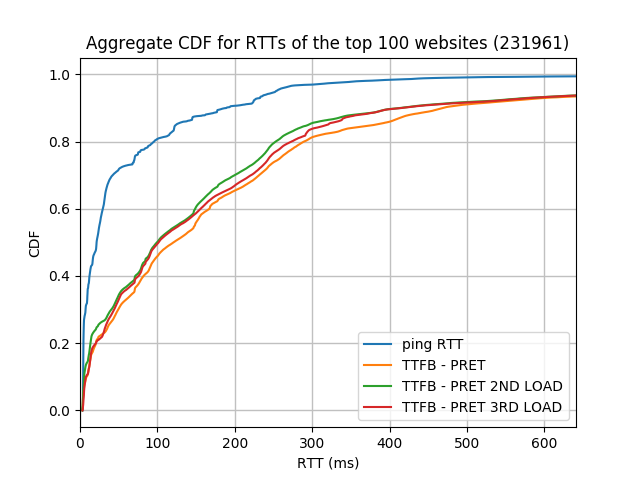
\includegraphics[width=0.41\textwidth]{fig/aggregategraph}
     \caption{Example figure}
      \label{fig:example}
\end{figure}

\section{Related work}
\label{sec:related-work}
% what other works are related to ours, and how.
Related work.

\section{Methodology}
\label{sec:methodology}

% explain what we've done in order to ensure reproducibility

Collection of data was conducted using two Python libraries: pyping and PycURL. Pyping is a pure Python ICMP ping implementation \cite{pypingdocs}. PycURL is a Python interface to libcurl, which is a client-side URL transfer library. PycURL allows one to fetch various objects identified by a URL: in our case, objects corresponding to the URLs of various websites hosted on servers across the world \cite{pycurldocs}.

First, we wanted to calculate the Round Trip Time (RTT) as measured by a calculation involving, at the highest level, a website's pretransfer time and time to first byte (TTFB): the RTT was calculated as the pretransfer time subtracted from the TTFB, both of which were obtained with PycURL. To do this, it is as simple as creating a new Curl Object from PycURL, setting the relevant options; i.e. the name of the website and the FOLLOWLOCATION to 1. Setting the FOLLOWLOCATION to 1 tells the library to follow any Location: header that the server sends as part of a HTTP header in a 3xx response. The Location: header can specify a relative or an absolute URL to follow. The library will issue another request for the new URL and follow new Location: headers all the way until no more such headers are returned \cite{curloptfollowlocationdocs}.

The next calculation we wanted to observe is the RTT on the second load of a website. This calculation has the same equation of RTT as described above, except with the appropriate second load of the pretransfer time and TTFB. In order to measure this, we took advantage of PycURL allowing for reuse of Curl Objects: one only needs to reset the relevant options identically to the first load and can then perform on the Curl Object. This process was repeated to calculate the RTT on the third load.

Finally, to get an ICMP ping time, it is as simple as using the ping function of pyping on a specified website's hostname.

The above network data; i.e. ICMP ping time and RTT of first, second, and third loads, were collected for a list of some of the most popular websites around the world at the time of writing this paper. A cron job was used to automate this collection of data to achieve a large sample size to analyze.

Data was plotted using the matplotlib library. In our analysis, we observed both aggregate data and site-specific data.

\section{Evaluation}
\label{sec:evaluation}

% present and analyze results.

Evaluation.

\section{Conclusions}
\label{sec:conclusions}

%\begin{itemize}
%\item Briefly restate the main points, results and contributions.
%\item Say what the lessons learned were
%\end{itemize}

% more synthesis than summary

Conclusions.



% The following two commands are all you need in the
% initial runs of your .tex file to
% produce the bibliography for the citations in your paper.
\bibliographystyle{IEEEtran}
%\small{
\bibliography{laspaper}
%\balancecolumns % must be placed in the laspaper.bbl right where you want the column break to occur
%}

%That's all folks!
\end{document}



